\documentclass[14pt]{matmex-diploma-custom}

\usepackage[table,xcdraw]{xcolor}
\usepackage{hyperref}	
\usepackage{enumitem}
\usepackage{listings}
\usepackage{color}
\usepackage{float}
\definecolor{urlcolor}{HTML}{0e0b61}



\hypersetup{
    colorlinks=true,
    linkcolor=black,
    filecolor=magenta,      
    urlcolor=urlcolor,
    pdftitle={Sharelatex Example},
    bookmarks=true,
    pdfpagemode=FullScreen,
}

\usepackage[utf8]{inputenc}

% Default fixed font does not support bold face
\DeclareFixedFont{\ttb}{T1}{txtt}{bx}{n}{12} % for bold
\DeclareFixedFont{\ttm}{T1}{txtt}{m}{n}{12}  % for normal

% Custom colors
\usepackage{color}
\definecolor{deepblue}{rgb}{0,0,0.5}
\definecolor{deepred}{rgb}{0.6,0,0}
\definecolor{deepgreen}{rgb}{0,0.5,0}

\usepackage{listings}

% Python style for highlighting
\newcommand\pythonstyle{\lstset{
language=Python,
basicstyle=\ttm,
otherkeywords={self},             % Add keywords here
keywordstyle=\ttb\color{deepblue},
emph={MyClass,__init__},          % Custom highlighting
emphstyle=\ttb\color{deepred},    % Custom highlighting style
stringstyle=\color{deepgreen},
frame=tb,                         % Any extra options here
showstringspaces=false            % 
}}


% Python environment
\lstnewenvironment{python}[1][]
{
\pythonstyle
\lstset{#1}
}
{}



\begin{document}
\filltitle{ru}{
    chair              = {Математическое обеспечение и администрирование информационных систем},
    title              = {Анализ решений задачи детекции лиц на изображениях в сфере киберкриминалистики},
    type               = {coursework},
    position           = {студентов},
    group              = {344},
    author             = {Федор Игоревич Жилкин},
    supervisorPosition = {доцент каф. СП СПбГУ, к.т.н.},
    supervisor         = {Ю.\,В. Литвинов},
    reviewerPosition   = {рук. отд. раз. ПО, ООО “Белкасофт”},
    reviewer           = {М.В. Виноградов},
}

%\filltitle{en}{
   % chair              = {Software and Administration of Information Systems},
 %  title              = {Classification of text content},
  %  type               = {coursework},
 %   author             = {Fedor Zhilkin},
  %  supervisorPosition = {Associate Professor},
  %  supervisor         = {Yurii Litvinov},
   % reviewerPosition   = {professor},
  %  reviewer           = {Timofey Bryksin},
%}

\maketitle
\tableofcontents

\section*{Введение} 
    
   Наша безопасность напрямую связана с успехами в области технического прогресса, ведь благодаря новым технологиям нам становится проще пресекать преступления и изолировать людей, совершивших злодеяние. Одним из важнейших средств безопасности являются камеры видеонаблюдения на улицах, в метро и в других общественных местах. Важно понимать, что количество информации, поступающей с этих камер, растет с каждым днем и автоматизация обработки полученных видео и фотографий становится всё более необходима.
    Решить эту проблему помогает автоматическое распознавание лиц для дальнейшей их верификации (определение того, что два лица на разных фотографиях принадлежат одному и тому же человеку), кластеризации (разбиение лиц на фотографиях по группам, каждая из которых соответствует одному человеку) и классификации (выяснение, принадлежит ли данное лицо человеку, находящемся в базе данных). \par
    Любая задача, связанная с лицами, начинается с их обнаружения на фотографиях или видео. Данная работа посвящена распознаванию лиц (face detection). В ней будут рассмотрены основные методы распознавания лиц, проведена сравнительная характеристика и будут выяснены лучшие решения этой задачи для работы в сфере криминалистики на основе двух ключевых факторов:
    
     \begin{itemize}
         \item эффективность решения в условиях слабой освещенности, наличия угла поворота лица и наличия вещей, частично закрывающих лицо; 
         \item по данным компании BelkaSoft у криминалистов чаще всего нет графических ускорителей, а тяжелые решения (например сверточные глубокие нейронные сети) требуют большой вычислительной мощности, что ведет к долгой работе на CPU, что подчеркивает важность быстродействия готового продукта.
     \end{itemize}
   
   Данная работа выполнена совместно с компанией Belkasoft, специализирующейся на создании программного обеспечения в сфере киберкриминалистики. Кроме того данное исследование выполнялось при участии студента Олега Чернявского, который занимается кластеризацией лиц (face clustering).
   
\section{Постановка задачи}

    Целью работы является обзор и сравнение уже существующих методов распознавания лиц на изображениях на основе факторов, приведенных во введении.
    По результатам исследования лучшее решение будет интегрировано в продукт BelkaSoft Evidence Center. Для успешного выполнения данной цели были поставлены следующие задачи:
    \begin{itemize}
        \item выбрать набор данных для тестирования решений; 
        \item рассмотреть существующие решения детектирования лиц; 
        \item создать тестирующую систему для сравнения решений;
        \item провести полное сравнение всех решений.
    \end{itemize}
    
\section{Выбор набора данных}    
    Для задачи обнаружения лиц в сфере киберкриминалистики необходимо выбрать набор изображений, обладающий определенными свойствами:
    \begin{itemize}
        \item окклюзия (возникает в ситуации, когда лицо частично прикрыто);
        \item лица, расположенные под разными углами;
        \item разная освещенность лиц;
        \item make-up (лицо чем-то разукрашено);
        \item разный размер лиц на изображениях (маленькие -- до 30х30 пикселей и большие -- больше 300х300 пикселей);
        \item разные эмоции на лицах. 
    \end{itemize}
    Существует достаточно много наборов данных, которые используются в задачах обнаружения лиц на изображениях. Вот некоторые из них:
    \begin{itemize}
        \item FDDB \cite{fddb};
        \item Wider Face \cite{dataset:WiderFaces};
        \item MAFA \cite{mafa};
        \item 4k face dataset \cite{4k}.
    \end{itemize}
    Все эти наборы данных используются в разных задачах детектирования лиц. Но для решения задачи успешного детектирования лиц в сфере киберкриминалистики нам необходимо наличие изображений, удовлетворяющих вышеназванным свойствам.Поэтому был выбран набор данных Wider Faces \cite{dataset:WiderFaces}. Это размеченный набор изображений, т.е. каждое лицо на каждом изображении имеет свои координаты, которые записаны в отдельном файле. Более того этот набор данных полностью удовлетворяет вышеназванным свойствам. В нем содержится около 12000 изображений, разбитых на три уровня сложности по каждому из параметров. Этот набор данных представляет особый интерес для криминалистов, так как чаще всего, изображения, полученные с камер видеонаблюдения имеют плохое качество, а лица на них могут быть чем-то прикрыты, плохо освещены или разрисованы.  
    Примеры изображений из этого набора данных приведены на Рис.1.
    
    \begin{figure}[h]
            \centering
            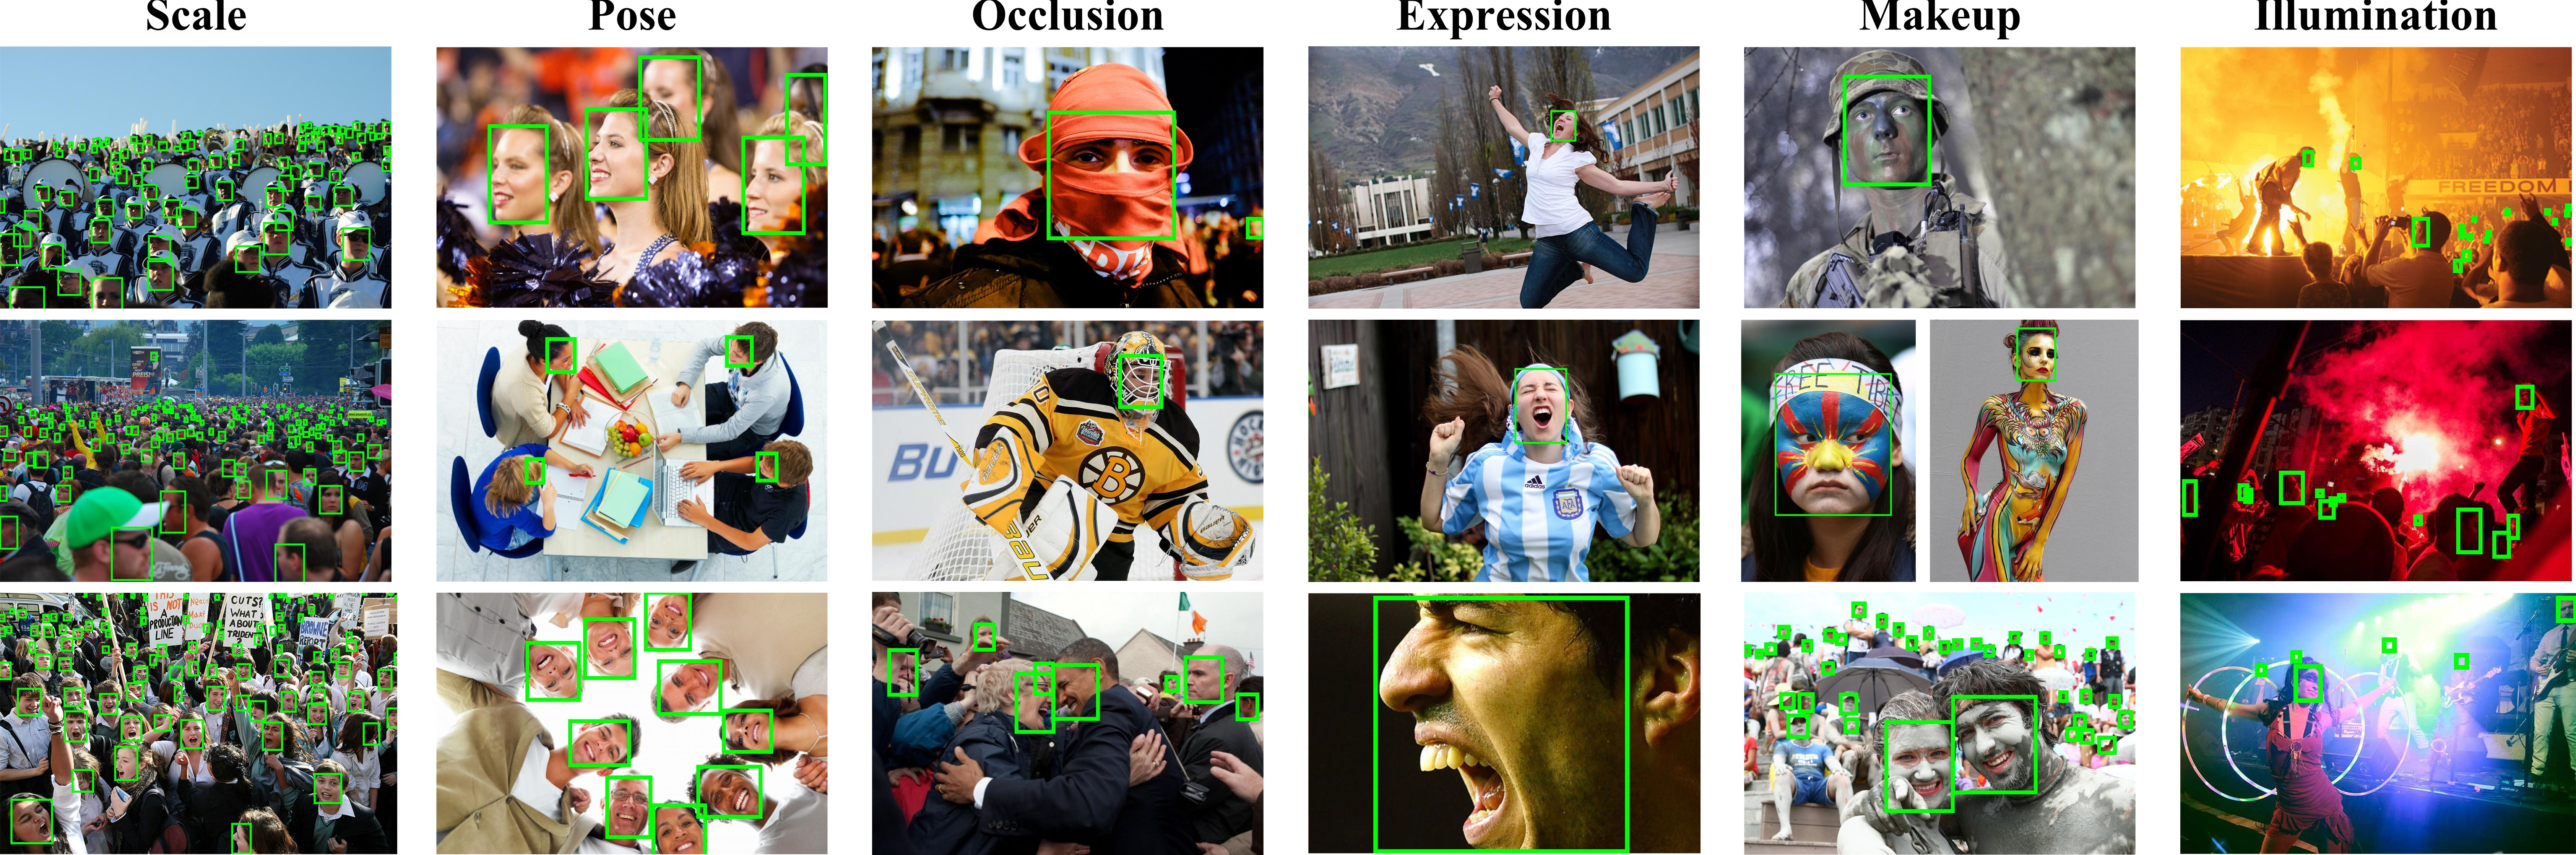
\includegraphics[width=1\textwidth]{images/intro.jpg}
            \caption{Набор данных Wider Faces, (источник: \url{https://arxiv.org/pdf/1511.06523.pdf}, дата обращения: 17.05.2020)}
    \end{figure}
    
\section{Выбор решений распознавания лиц}
    Выбирать решения будем, опираясь на следующие факторы:
    \begin{itemize}
        \item быстрота при работе на CPU;
        \item относительная популярность решений в индустрии;
        \item качество работы решений.
    \end{itemize}
    Поскольку продукт BelkaSoft Evidence Center работает под платформой .NET, то для тестирования были выбраны решения, которые уже реализованы под данной платформой и удовлетворяют вышеописанным факторам:
    \begin{itemize}
        \item каскады Хаара и LBP;
        \item гистограмма ориентированных градиентов (HOG);
        \item Single-Shot-Multibox Detector (SSD);
        \item FaceNet's Multi-Task Cascaded Neural Network (MTCNN);
        \item Maximum-Margin Object Detector (MMOD).
    \end{itemize}
    
    Также были выбраны три решения, показавшие лучшие результаты на выбранном наборе данных Wider Faces:
    \begin{itemize}
        \item Dual Shot Face Detector (DSFD);
        \item Selective Refinement Network for High Performance Face Detection (SRN);
        \item Accurate Face Detection for High Performance (AInnoFace).
    \end{itemize}
    
    Последние три решения -- специально обученные на этом же наборе изображений нейронные сети. Они имеют хорошие результаты (будут приведены ниже), но они не были протестированы на других наборах данных, поэтому объективную оценку этим решениям в контексте текущей задачи дать нельзя. Эти решения приведены лишь для сравнения с результатами вышеописанных решений. В дальнейшем планируется реализовать эти решения под платформой .NET и протестировать на других наборах данных.


\section{Схема тестирования}

Окончательная оценка решений будет определяться двумя тестами:
\begin{itemize}
    \item тест на точность решения на выбранном наборе данных;
    \item тест на скорость работы на CPU.
\end{itemize}
 
 \subsection{Метрика IoU}
    Введем метрику степени пересечения между двумя ограничивающими рамками. Это необходимо для того, чтобы понимать, правильно ли алгоритм обнаружил лицо на изображении. IoU (Intersection-over-Union) считается следующим образом:
    $$IoU = \frac{Intersection\_Area}{Union\_Area}$$ \par
    Если IoU от набора реальных координат лица ($ground\_truth$) и набора координат, полученного из алгоритма ($predicted\_vector$), больше или равно 0.5, то говорим, что этот полученный набор координат -- действительно правильно обнаруженное лицо. Примеры IoU метрик можно увидеть на Рис.2. 
    
  \begin{figure}[h]
            \centering
            \includegraphics[width=0.8\textwidth]{images/IoU.png}
            \caption{Метрика Intersection-over-Union (источник: \url{https://habr.com/ru/company/jetinfosystems/blog/498294/}, дата обращения: 17.05.2020)}
    \end{figure}
 
 
 \subsection{Классы TP, FP, FN}
    Для построения метрик введем классы True-Positive (TP), False-Positive (FP), False-Negative (FN). Как показано на Рис.3, у нас есть три варианта для результатов, полученных алгоритмом: 
    \begin{itemize}
        \item при $IoU(ground\_truth, predicted\_vector) \geq 0.5$ -- True-Positive (лицо обнаружили, как минимум, наполовину);
        \item при $IoU(ground\_truth, predicted\_vector) < 0.5$ -- False-Positive (вектор, не являющееся ground-truth лицом);
        \item все остальные лица, не обнаруженные алгоритмом -- False-Negative.
    \end{itemize}
 
 \begin{figure}[h]
            \centering
            \includegraphics[width=1\textwidth]{images/tp.png}
            \caption{Классы TP, FP, FN (источник: Набор данных Wider Faces)}
    \end{figure}
    
 \subsection{Метрики Recall, Precision, F-мера}
    Для оценки точности работы алгоритмов введем следующие метрики:
    \begin{itemize}
        \item $Recall = \frac{TP}{TP+FN}$; 
        \item $Precison = \frac{TP}{TP+FP}$;
        \item $F_\beta = (1+\beta^2)\cdot\frac{Precision\cdot Recall}{(\beta^2\cdot Precision) + Recall}$.
    \end{itemize}
    Recall показывает, какую долю лиц из всех лиц на изображении нашел алгоритм. Precision можно интерпретировать как долю лиц, названных детектором лицами и при этом действительно являющимися лицами. Если наш детектор будет обнаруживать все как лицо, то Recall будет стремиться к единице, а Precision -- к нулю. Зеркальная ситуация (та, в которой детектор ничего не обнаруживает) дает нам обратные результаты (Recall стремится к нулю, Precision -- к единице).
    Получается, что невозможно оценить качество работы алгоритма только лишь по одному из этих параметров. Поэтому вводится метрика F-мера. Она представляет собой среднее гармоническое Precision и Recall. F-мера позволяет точно определить качество работающего алгоритма. Именно на эту метрику будем ссылаться при тестировании наших решений.
    
 \subsection{Алгоритм тестирования}
 
 Для тестирования решений была выбрана легкая часть набора изображений по параметру Scale, где каждое изображение содержит лица, размером не меньшие, чем 300x300 пикселей. Далее для каждого изображения получаем реальные координаты лиц (ground-truth векторы) и координаты, полученные с помощью решения (predicted векторы). Затем с помощью метрики IoU заполняем классы TP, FP, FN. После вычисляем метрики Recall, Precision, F-мера. Схематично алгоритм тестирования изображен на Рис.4. Таким образом, первая часть тестирования закончена.
 
  \begin{figure}[h]
            \centering
            \includegraphics[width=0.6\textwidth]{images/diag.png}
            \caption{Алгоритм тестирования решений}
    \end{figure}
    
    Вторая часть тестирования заключается в проверке скорости работы решения. Для этого возьмем изображение 300x300 пикселей и запустим на нем решение 10000 раз. Посчитаем среднюю скорость обработки изображения и дисперсию (минимальное и максимальное время). После этого выберем лучшее решение по этим двум тестам. 
 
\section{Тестируемые решения}

    Поскольку данная работа носит обзорный характер, мы не будем подробно рассматривать все шаги каждого алгоритма, а остановимся на самых важных, благодаря которым можно понять общую концепцию решения.
    \subsection{Каскады Хаара}
        Каскадный классификатор Хаара, впервые описанный в 2001 году в оригинальной статье  \cite{haar:cascade}, представляет собой особый случай ансамблированного обучения  \cite{wiki:ensemble}, называемый ускорением (boosting). Как правило, он основан на классификаторах Adaboost \cite{wiki:ada}.
        Существует алгоритм, называемый <<алгоритмом Виолы-Джонса>>, который включает в себя все этапы, необходимые для обнаружения лица:
        \begin{itemize}
            \item выбор характеристик (признаков) Хаара; 
            \item интегральное представление изображения;
            \item Adaboost Training;
            \item каскадный классификатор.
        \end{itemize}
        Рассмотрим некоторые шаги алгоритма: \\
    \textbf{Выбор характеристик Хаара.} \\ 
        Есть некоторые общие черты, которые мы находим на человеческих лицах:
        \begin{itemize}
            \item темная область глаз по сравнению с областью щек;
            \item яркая область переносицы по сравнению с областью глаз;
            \item какое-то конкретное расположение глаз, рта, носа.
        \end{itemize}
        Процесс извлечения этих характеристик продемонстрирован на Рис. 5.
    
        \begin{figure}[h]
            \centering
            \includegraphics[scale=0.5]{images/haar.jpg}
            \caption{Извлечение характеристик (feature extraction) (источник: \url{https://www.cs.cmu.edu/~efros/courses/LBMV07/Papers/viola-cvpr-01.pdf}, дата обращения: 17.05.2020)}
        \end{figure}
        
        В этом примере первая характеристика измеряет разницу в интенсивности между областью глаз и областью щек. Значение характеристики вычисляется путем суммирования пикселей в черной области и вычитания пикселей в белой области.
        $$RectangleFeature = \sum{pixels_{blackarea}} - \sum{pixels_{whitearea}}$$ \par
        Затем мы применяем эту характеристику как сверточное ядро по всему нашему изображению. Вычислять прямоугольные характеристики, используя принцип интегрального изображения, получается намного быстрее, поэтому следующий шаг после выбора характеристик -- интегральное представление изображения \cite{v:j}.
        
        Существует несколько типов прямоугольников (изображены на Рис. 6), которые можно применять для извлечения характеристик Хаара. 
        
        \begin{figure}[h]
            \centering
            \includegraphics[scale=0.9]{images/haar_rectangles.jpg}
            \caption{Прямоугольники Хаара (Haar's rectangles) (источник: \url{https://www.cs.cmu.edu/~efros/courses/LBMV07/Papers/viola-cvpr-01.pdf}, дата обращения: 17.05.2020)}
        \end{figure}
        
        Теперь, когда характеристики выбраны, мы применяем их к набору обучающих изображений, используя классификацию Adaboost, которая представляет собой набор слабых классификаторов, для создания точной ансамблированной модели (ansamble model).\\
    \textbf{Каскадный классификатор} \\ 
        На изображении большая часть изображения -- это область без лица. Придавать одинаковую важность каждой области изображения не имеет смысла, поскольку мы должны сосредоточиться на областях, которые, скорее всего, содержат лицо. 
        Ключевая идея состоит в том, чтобы не рассматривать области изображения, которые не содержат граней (областей резкой смены интенсивности цвета). Поскольку задача состоит в том, чтобы правильно идентифицировать лицо, мы хотим минимизировать количество ложных отрицательных результатов, при которых области, которые содержат лицо не были идентифицированы как области с лицом.
        
        Ряд классификаторов применяется к каждой области изображения. Эти классификаторы являются простыми деревьями решений:
        \begin{itemize}
            \item если первый классификатор положительный, мы переходим ко второму;
            \item если второй классификатор положительный, мы переходим к третьему;
            \item ...
        \end{itemize}
        Любой отрицательный результат в некоторой точке приводит к отклонению области как потенциально содержащей лицо. Первоначальный классификатор исключает большинство отрицательных примеров при низких вычислительных затратах, а следующие классификаторы устраняют дополнительные отрицательные примеры, но требуют больших вычислительных усилий. Схематично этот процесс изображен на Рис.7.
        
            \begin{figure}[h]
                    \centering
                    \includegraphics[scale=0.8]{images/1328.jpg}
                    \caption{Каскад (Haar's cascade) (источник: \url{https://habr.com/ru/post/208092/}, дата обращения: 17.05.2020)}
            \end{figure}    
        
            
    \subsection{Гистограмма ориентированных градиентов}
        Работу HOG \cite{hog} можно описать следующими шагами:
        \begin{itemize}
            \item предварительная обработка изображения, включая изменение размера и нормализацию цвета;
            \item вычисление вектора градиентов каждого пикселя, а также его величину и направление;
            \item Разделение изображения на множество ячеек размером 8х8 пикселей. В каждой ячейке значения магнитуд этих 64 ячеек сгруппированы и кумулятивно добавлены в 9 сегментов без учета направления ($0^{\circ}-180^{\circ}$ вместо $0^{\circ}-360^{\circ}$), то есть построена гистограмма направленных градиентов.
        \end{itemize} \par
        
        Конечным шагом в распознавании объектов с использованием HOG является классификация дескрипторов при помощи системы обучения с учителем \cite{wiki:supervised}. Создатели алгоритма использовали метод опорных векторов (SVM, Support Vector Machine) \cite{wiki:SVM}.
    
    \subsection{Single-Shot-Multibox Detector}
        Данный метод, Single-Shot-Multibox Detector (SSD), впервые описанный в 2016 году в оригинальной статье \cite{SSD}, позволяет обнаруживать объекты на изображениях, используя только одну глубокую сверточную нейронную сеть. При использовании этого подхода выходное пространство границ обнаруженных объектов (space of bounding boxes) разбивается на набор базовых прямоугольников с различными соотношениями сторон. В качестве предсказания алгоритм выдает числа, определяющие степень уверенности в присутствии той или иной категории объектов в каждом из базовых прямоугольников. Также производится корректировка границ с целью лучшего покрытия объекта на изображении. 
            В названии  “Single Shot MultiBox Detector”:
            \begin{itemize}
                \item Single Shot означает, что задачи локализации и классификации объектов выполняются за один проход сети;
                \item MultiBox -- методика поиска ограничивающего прямоугольника;
                \item Detector --  нейронная сеть, которая работает как детектор объектов.
            \end{itemize}
            
            \begin{figure}[h]
                    \centering
                    \includegraphics[width=1\textwidth]{images/ssd.png}
                    \caption{Схема работы SSD (источник: \url{http://dx.doi.org/10.1007/978-3-319-46448-0_2}, дата обращения: 17.05.2020)}
            \end{figure}   
            Рис.8 демонстрирует схему работы данного подхода. К входному изображению применяется некоторое количество сверточных слоев, причем часть из этих слоев взята из модели VGG16 \cite{VGG:16}. Пространственная размерность изображения убывает после каждого слоя, доходя до единицы. Далее к промежуточным результатам применяется блок <<Detector and classifier>>, на выходе которого имеем детекцию, т.е. прямоугольники с классом. Затем эти детекции подаются на вход алгоритму Fast Non-Maximum Suppression (Fast NMS) \cite{non:maximum}. Этот алгоритм объединяет все прямоугольники для получения финального результата.
            
    \subsection{Local Binary Patterns}
            Local Binary Patterns (LBP) -- простой оператор, используемый для классификации текстур. Впервые был описан в оригинальной статье \cite{lbp} в 1996 году. Концепцию работы этого решения можно изложить следующим образом:
            \begin{itemize}
                \item выбираются радиус и количество точек (см. Рис.9). Далее будем считать LBP на основе восьми смежных точек;
                \begin{figure}[h]
                    \centering
                    \includegraphics[width=1\textwidth]{images/lbpdots.png}
                    \caption{Выбор точек для построения LBP (источник: \url{https://habr.com/ru/post/280888/}, дата обращения: 17.05.2020)}
                 \end{figure}  
                 
                \item далее необходимо пронумеровать выбранные точки;
                \item затем вычисляем разность значений яркости между каждым из крайних пикселей и центральным;
                \item если разность отрицательная (яркость убывает), записываем на месте соседа единицу, если неотрицательная -- ноль;
                \item построим гистограмму по полученным клеткам (см. Рис.10).
                    \begin{figure}[h]
                        \centering
                        \includegraphics[width=1\textwidth]{images/lbphist.png}
                        \caption{Полученная гистограмма смены интенсивности в области (источник: \url{https://habr.com/ru/post/280888/}, дата обращения: 17.05.2020)}
                    \end{figure}  
            \end{itemize}
            
            Полученное двоичное число называется Local Binary Pattern. По существу, биты дескриптора -- это знаки производных яркости по направлениям. Последним шагом алгоритма будет подача полученных гистограмм на вход метода опорных векторов (SVM). 
            
    \subsection{Max-Margin Object Detection} 
    Большинство методов обнаружения объектов работают путем применения
    двоичного классификатора к определенным областям изображения, при этом обнаружение на перекрывающихся областях удаляется. Поскольку число возможных областей в наборах данных
    изображений даже умеренного размера чрезвычайно велико, классификатор
    обычно обучается только на подмножестве этих областей. Это позволяет избежать
    вычислительных трудностей при работе со всем набором областей, однако это приводит к неоптимальной производительности детектора.
    Метод Max-Margin Object Detection (MMOD) \cite{mmod} не выполняет подвыборку, а
    оптимизирует все области. MMOD может быть использован для улучшения
    методов обнаружения объектов, таких как HOG или каскадный классификатор Хаара.
    
    
    \subsection{Multi-Task Cascaded Neural Network}
    Метод обнаружения и выравнивания лиц Multi-Task Cascaded Neural Network (MTCNN) описан в статье \cite{mtcnn} в 2016 году. 
    Конвейер каскадного метода обнаружения лиц делится на три основные стадии:
    \begin{itemize}
        \item используем сверточную сеть, сеть предложений (P-Net), чтобы получить области-кандидаты и их ограничивающие рамки. Затем мы используем оцененные векторы регрессии ограничивающего прямоугольника для калибровки кандидатов. После этого мы используем алгоритм Non-Maximum Suppression (Fast NMS) \cite{non:maximum} для слияния сильно перекрывающихся кандидатов (см. Рис.11);
            \begin{figure}[H]
                        \centering
                        \includegraphics[width=1\textwidth]{images/1satge.png}
                        \caption{Поиск областей-кандидатов (источник: \url{https://arxiv.org/ftp/arxiv/papers/1604/1604.02878.pdf}, дата обращения: 17.05.2020)}
            \end{figure} 
        \item все области-кандидаты подаются на другой слой CNN, называемый Refine Network (R-Net), который дополнительно отклоняет большое количество ложных кандидатов, выполняет калибровку с помощью регрессии ограничивающего прямоугольника. Далее происходит слияние кандидатов с помощью алгоритма NMS (см. Рис.12);
            \begin{figure}[H]
                        \centering
                        \includegraphics[width=1\textwidth]{images/2stage.png}
                        \caption{Уточнение областей-кандидатов (источник: \url{https://arxiv.org/ftp/arxiv/papers/1604/1604.02878.pdf}, дата обращения: 17.05.2020)}
            \end{figure} 
            \item третья стадия похожа на вторую, но на этой стадии мы стремимся описать лицо более подробно. В частности, сеть будет выводить на экран пять лицевых ориентиров (нос, глаза, уголки рта) (см. Рис. 13).
            \begin{figure}[H]
                        \centering
                        \includegraphics[width=1\textwidth]{images/3stage.png}
                        \caption{Вывод окончательных границ и точек-ориентиров лица (источник: \url{https://arxiv.org/ftp/arxiv/papers/1604/1604.02878.pdf}, дата обращения: 17.05.2020)}
            \end{figure}
    \end{itemize}
    
    %\clearpage
    \section{Результаты тестирования}
        \subsection{Результаты лучших решений}
        Рис. 14 демонстрирует результаты решений, показавших лучшие результаты на наборе данных Wider Faces. Видно, что F-мера трех лучших решений близка к единице, что говорит об очень неплохой точности алгоритмов. В дальнейшем планируется интегрировать эти решения под платформу .NET и протестировать на других наборах данных. Далее будем оценивать наши остальные решения, исходя из того, что знаем лучшие результаты.
        
            \begin{figure}[H]
                        \centering
                        \includegraphics[width=1\textwidth]{images/chart.png}
                        \caption{График <<Face Detection on Wider Faces>> (источник: \url{https://paperswithcode.com/paper/wider-face-a-face-detection-benchmark}, дата обращения: 17.05.2020)}
           \end{figure} 
        
        \subsection{Результаты решений, интегрированных под платформу .NET}
                \begin{table}[H]
                \centering 
\begin{tabular}{|l|l|l|l|}
\hline
                              & \cellcolor[HTML]{CBCEFB}Recall & \cellcolor[HTML]{CBCEFB}Precision & \cellcolor[HTML]{CBCEFB}F-Score \\ \hline
\cellcolor[HTML]{CBCEFB}LBP   & 0.29                           & 0.86                              & 0.43                            \\ \hline
\cellcolor[HTML]{CBCEFB}HOG   & 0.38                           & 0.95                              & 0.54                            \\ \hline
\cellcolor[HTML]{CBCEFB}Haar  & 0.45                           & 0.91                              & 0.60                            \\ \hline
\cellcolor[HTML]{CBCEFB}MMOD  & 0.52                           & 0.86                              & 0.65                            \\ \hline
\cellcolor[HTML]{CBCEFB}SSD   & 0.82                           & 0.66                              & 0.73                            \\ \hline
\cellcolor[HTML]{CBCEFB}MTCNN & 0.86                           & 0.89                              & 0.87                            \\ \hline
\end{tabular}
\caption{Результаты существующих решений под .NET}
\end{table}
    
    Как видно из таблицы 1, лучшие результаты показывают MTCNN и SSD. Однако SSD имеет достаточно низкий параметр Precision, что вызвано высоким содержанием False-Positive обнаружений. 
        
        \subsection{Результаты тестирования скорости при работе на CPU}
          Скорость будем тестировать на изображении размером 300х300. Каждый алгоритм обработает изображение 10000 раз. \\ 
        \textbf{Hardware:}
        \begin{itemize}
            \item Processor : Intel Core i7 6850K – 6 Core;
            \item RAM : 32 GB;
            \item GPU : NVIDIA GTX 1080 Ti with 11 GB RAM;
            \item OS : Ubuntu 16.04 LTS;
            \item Programming Language : C\#.
        \end{itemize}
        
        \begin{figure}[H]
                        \centering
                        \includegraphics[width=1\textwidth]{images/meta-chart.png}
                        \caption{Средняя скорость работы с минимальным и максимальным временем}
       \end{figure} 
        
        Самое лучшее решение по свойству быстродействия -- LBP. Также довольно быстро работают каскады Хаара, SSD и HOG.
        
        \subsection{Тест на поворот лица}
        Рис. 16 показывает как разные решения справляются с ситуацией, в которой лицо повернуто на некоторый градус. Лучше всего с этой задачей справляется SSD. Это решение обнаруживает лицо с углом поворота вплоть до $180^{\circ}$. 
        \begin{figure}[H]
                        \centering
                        \includegraphics[width=1\textwidth]{images/0011.png}
                        \caption{Обнаружение лица под углом}
       \end{figure}
        
        \subsection{Тест на окклюзию}
        Тест на окклюзию изображен на Рис. 17. Лучшие результаты показывают решения SSD и MTCNN. Они обнаруживают лицо даже, когда оно прикрыто наполовину.
        \begin{figure}[H]
                        \centering
                        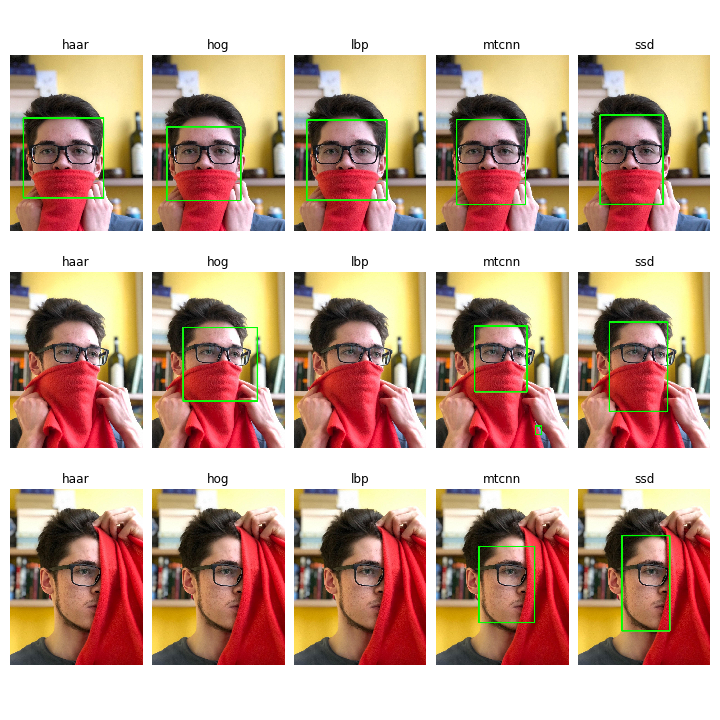
\includegraphics[width=1\textwidth]{images/scarf_test.png}
                        \caption{Обнаружение частично прикрытого лица}
       \end{figure}
        
 \newpage
 \section{Результаты}
    Исходя из поставленных целей и задач, были получены следующие результаты:
    \begin{itemize}
        \item создана система для тестирования различных решений;
        \item рассмотрены существующие решения детектирования лиц на изображениях;
        \item проведено полное сравнение всех решений и выбрано лучшее -- Single-Shot-Multibox Detector;
        \item \url {https://github.com/Feodoros/BelkaFaces/blob/master/WiderFaces.ipynb}.
    \end{itemize}
\newpage
\setmonofont[Mapping=tex-text]{CMU Typewriter Text}
\bibliographystyle{ugost2008ls}
\bibliography{diploma.bib}
\end{document}